\documentclass[11pt,pdftex,dvipsnames,usenames,helvetica]{beamer}
\setbeameroption{show notes}
\usepackage[round]{natbib}
\usepackage{textcomp}
\usepackage{amsmath}
\usepackage{amssymb}
\usepackage{graphicx}
\DeclareGraphicsExtensions{.ps,.eps,.pdf,.jpg,.png}
\usefonttheme[onlymath]{serif}
\usepackage[cmintegrals,cmbraces]{newtxmath}
\usetheme{default}
\usecolortheme{dove}

\usepackage{cancel}
\usepackage{tikz}
\usepackage[english]{babel}

\usepackage{verbatim}
\usepackage{color}
\usepackage{pgf} %portable graphics format
\usepackage[autobold]{statex2}
\mode<presentation>
{
  %\usetheme{Warsaw}
  % or ...
  \setbeamercovered{transparent}
  % or whatever (possibly just delete it)

  \setbeamertemplate{navigation symbols}{}
  \usefonttheme[onlysmall]{structurebold}
  %\usefonttheme{structurebold}
}
\addtobeamertemplate{navigation symbols}{}{%
    \usebeamerfont{footline}%
  \setbeamertemplate{navigation symbols}{}
    \usebeamercolor[fg]{footline}%
    \hspace{1em}%
    \insertframenumber/\inserttotalframenumber
}
\newcommand*{\red}[1]{\textcolor{red}{#1}}
\newcommand*{\blue}[1]{\textcolor{blue}{#1}}

\begin{document}
\boldmath
% 0. Intro

\begin{frame}
\frametitle{Graduate School Class Reminders}

\begin{itemize}
% \item Keep your facial covering on, including over your nose
\item Maintain six feet of distancing
\item Please sit in the same chair each class time
\item Observe entry/exit doors as marked
\item Use hand sanitizer when you enter/exit the classroom
\item Use a disinfectant wipe/spray to wipe down your learning space
  before and after class
\item Media Services: 414 955-4357 option 2
%\item START RECORDING
\end{itemize}

\end{frame}

\begin{frame}
\frametitle{Documentation on the web}

\begin{itemize}
\item CRAN: \url{http://cran.r-project.org}
\item R manuals: \url{https://cran.r-project.org/manuals.html}
\item SAS: \url{http://support.sas.com/documentation}
\item Step-by-Step Programming with Base SAS 9.4 (SbS): \\
\url{https://documentation.sas.com/api/docsets/basess/9.4/content/basess.pdf}
\item SAS 9.4 Programmer s Guide: Essentials (PGE): \\
\url{https://documentation.sas.com/api/docsets/lepg/9.4/content/lepg.pdf}
\item Wiki: \url{https://wiki.biostat.mcw.edu} 
\textcolor{red}{(MCW/VPN)}
\end{itemize}

\end{frame}

\begin{frame}[fragile]
\frametitle{Multi-threading example: the Mandelbrot set}

\begin{itemize}
\item To study multi-threading, a computational
example is helpful that takes some time to complete, but NOT too much time
%\item Here we use an example known as the Mandelbrot set 
\item Complex numbers are of the form: $c=x+y\mathrm{i}$
where $\mathrm{i}^2=-1$\\
$Re(c)=x, Im(c)=y,\ Mod(c)=\sqrt{x^2+y^2}$\\
R functions: Real part {\tt Re}; Imaginary {\tt Im}; and Modulus {\tt Mod}
\item Multiplying two complex numbers together has
  different behavior than real numbers, e.g., the product's modulus 
 need NOT be greater than the terms multiplied
  even if both quantities have real and imaginary parts greater than one
\item The Mandelbrot set contains the following $c=x+y\mathrm{i}$ values
\item Suppose $d_0=0+0\mathrm{i}$
\item Iterate the relation: $d_{n}=d_{n-1}^2+c$ for $n=1, \dots, N$ 
\item It is known that if $Mod(d_n)>2$, then $c$ is NOT in the set
\item How many iterations, $n$, does it take $d_n$ to
  diverge for each $c$?
\item Heat map: $Re(c)$, $Im(c)$ and $n$ are the $x$, $y$ and $z$ axes
\end{itemize}
Myles Harrison at \url{http://everydayanalytics.ca}
\end{frame}

\begin{frame}[fragile]
\frametitle{HW: the Mandelbrot set}

\begin{itemize}
\item Use multi-threading to speed up the calculations
\item Divide up the plane into 4 quadrants
\item Submit each quadrant in a separate thread 
\end{itemize}
\end{frame}

\begin{frame}[fragile]
\frametitle{Multi-threading and symmetric multi-processing}

\begin{itemize}
\item Multi-threading and symmetric multi-processing are\\
\textcolor{red}{advanced technology} that are 
\textcolor{blue}{surprisingly easy to use today}
\item Multi-threading emerged quite early in the digital
  computer age with the groundwork laid in the 1960s
\item In 1961, Burroughs released the B5000 which was the first
  commercial hardware capable of multi-threading
\item The B5000 performed asymmetric multiprocessing which is commonly
  employed in modern hardware like numerical co-processors and/or
  graphical processors today
\item In 1962, Burroughs released the D825 which was the first
  commercial hardware capable of symmetric multiprocessing (SMP) with
  CPUs
\item In 1967, Gene Amdahl derived the theoretical limits for
  multi-threading which came to be known as Amdahl's law
\item If $B$ is the number of CPUs and $b$ is the fraction
of work that can't be parallelized, then the gain due to
multi-threading is $((1-b)/B+b)^{-1}$
\end{itemize}
\end{frame}

\begin{frame}[fragile]
\frametitle{Amdahl's law: $((1-b)/B+b)^{-1} \where b \in \{0.025, 0.1\}$}
%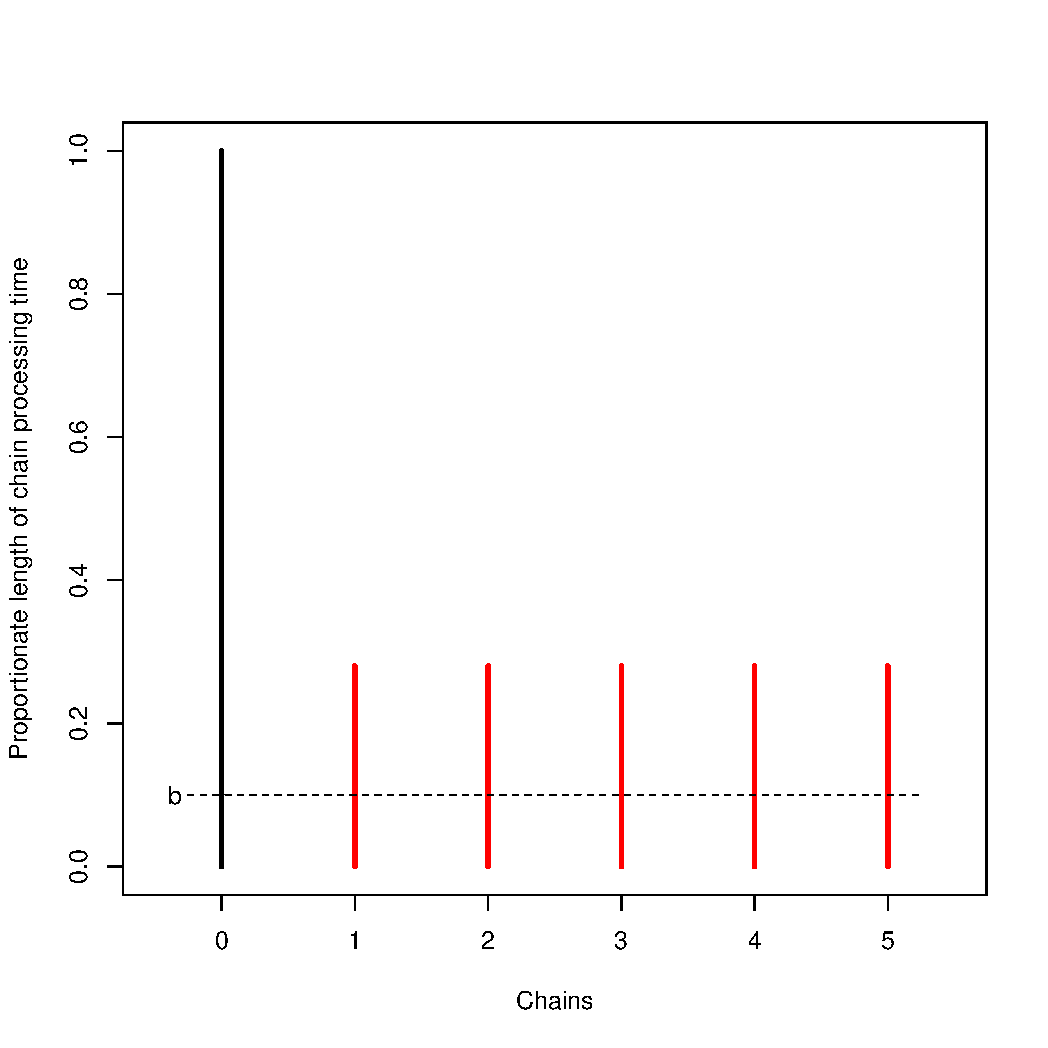
\includegraphics[scale=0.48]{parallel.pdf}
\begin{center}
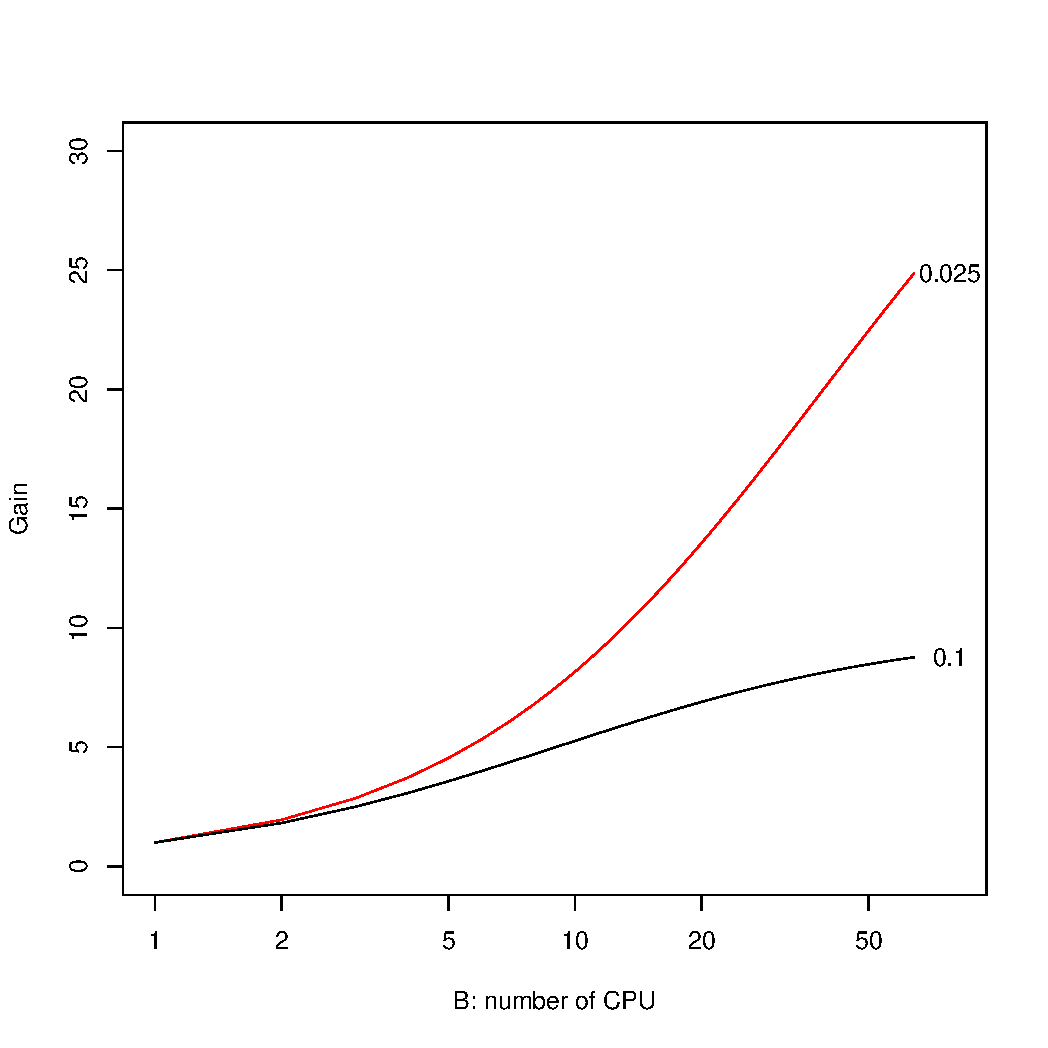
\includegraphics[scale=0.5]{amdahl.pdf}
\end{center}
\end{frame}


\begin{frame}[fragile]
\frametitle{Multi-threading and symmetric multi-processing}

\begin{itemize}
%\item Fast-forward to the modern era of multi-threading
\item Hardware and
software architectures in current use directly, and indirectly,
led to wide availability of multi-threading today
\item In 2000, Advanced Micro Devices (AMD) created AMD64\\
  new 64-bit x86 instructions to coexist with 16-/32-bit x86 
%legacy instructions
\item An important advance since 64-bit math is capable of addressing
  vastly
  more memory than 16-/32-bit\\
  ($2^{64}$ vs.\ $2^{16}$ or $2^{32}$) since multi-threading
  inherently requires more memory resources
\item In 2003, version 2.6 of the Linux kernel incorporated full SMP
  support: prior Linux kernels had none/limited/crippled support
% \item From 2005 to 2011, AMD released a series of Opteron chips
% with multiple cores for multi-threading: 2 cores in 2005, 4 cores in
% 2007, 6 cores in 2009, 12 cores in 2010 and 16 cores in 2011.
\item From 2008 to 2010, Intel brought to market AMD64 Xeon chips with
  their hyper-threading technology that allows each core to issue two
  instructions per clock cycle: 4 cores\\ (8 threads) in 2008 and 8
  cores (16 threads) in 2010
\item Today, most off-the-shelf hardware available features 1 to 4
  CPUs each of which is capable of multi-threading: in the span of a
  few years, multi-threading rapidly trickled down from higher-end
  servers to mass-market desktops and laptops
\end{itemize}
\end{frame}

\begin{frame}[fragile]
\frametitle{Multi-threading with {\tt parallel} package}

\begin{itemize}
\item The {\tt mcparallel} function uses \textcolor{blue}{\it forking}
  to facilitate multi-threading (forking is NOT available on Windows)
\item {\it Fork} is an operation where a process creates a copy of itself
\item A {\it forked} R {\it child} process has memory address {\it
    pointers} to all of the objects known to the {\it parent} such as
  loaded packages, function definitions, data frames, etc.
\item But, these {\it shared} objects are NOT copied into memory
  for each child: that would be a huge waste of resources!
\item Each child has a memory address {\it pointer} to these objects
\item However, R has a \textcolor{red}{\it copy on write} philosophy
\item If a child writes to an object owned by the parent, a copy
is made for the child while the parent retains the original
\item This is convenient, but can be dangerous with multiple threads
\item For example, if this is a big object, now that object has
multiple instances which might consume a lot of memory 
\end{itemize}
\end{frame}


\begin{frame}[fragile]
\frametitle{The {\tt detectCores} function}

\begin{itemize}
\item returns the number of threads that the computer is capable of
\item the number of {\it threads} rather than the number of {\it cores}
since they are not necessarily one-to-one
\item {\tt detectCores()} will occasionally return {\tt NA}
\item {\tt detectCores(TRUE)} {\it might} fix that
\item often, just calling {\tt detectCores()} again will work
\item however, this is an annoying bug/feature
\item these are \textcolor{red}{sporadic} failures
rather than \textcolor{blue}{reproducible} failures
\item \textcolor{blue}{reproducible} failures can typically
be {\it debugged}, but often \textcolor{red}{sporadic} cannot
\end{itemize}
\end{frame}

\begin{frame}[fragile]
\frametitle{The {\tt mcparallel} function and \textcolor{red}{nice}}
\begin{verbatim}
library(parallel) ## an example of multi-threading
library(tools)
for(i in 1:mc.cores) mcparallel({psnice(value=19); expr})
obj.list = mccollect() 
...
\end{verbatim}
\begin{itemize}
\item {\tt expr} is processed {\tt mc.cores} times
  each in their own threads
\end{itemize}
Paraphrasing the {\tt psnice} documentation\\
%\begin{quote}
Unix schedules processes to execute according to their priority.\\  Priority
is assigned values from 0 to 39 with 20 being the normal priority and
(counter-intuitively) larger numeric values denoting lower priority.
Adding to the complexity, there is a {\it nice} value:\\ the amount by
which the priority exceeds 20.  Processes with higher nice values will
receive less CPU time than those with normal priority.  Generally,
processes with nice value 19 are only run when the system would
otherwise be idle \textcolor{blue}{to enhance system interactivity}.
%\end{quote}
\end{frame}

\begin{frame}[fragile] 
\frametitle{The {\tt mccollect} function}
\begin{itemize}
\item {\tt mccollect} returns a list of return values from each thread
\item in my experience, these are returned last in, first out (LIFO)\\ 
the reverse from what we might have expected
\item occasionally, a \textcolor{red}{sporadic} failure in one, or
  more, of the threads\\
failed component(s) are missing from the list of return values
%\item so, the length of {\tt length(obj.list) $<$ mc.cores}
\item if it is sporadic: re-running without any changes will succeed
% \item often, re-running the job will return all {\tt mc.cores} list
%   components without any changes to the R program
\item {\tt class(obj)[1]!=type} is likely an error message so return it
\end{itemize}
\begin{verbatim}
obj.list = mccollect() ## last in, first out
obj = obj.list[[1]]
if(mc.cores==1 | class(obj)[1]!=type) {
    return(obj)
} else {
    m = length(obj.list)
    if(mc.cores!=m) 
        warning(paste0("The number of items is only ", m))
    ...
}
\end{verbatim}
\end{frame}

\begin{frame}[fragile] 
\frametitle{The {\tt mcparallel} function and random number generation}
\begin{itemize}
\item We want each thread to have its own {\it stream} of random numbers
that is reproducible
\item There is a special random number generator for this purpose
\item L'Ecuyer's combined multiple-recursive generator (CMRG)
\end{itemize}
\begin{verbatim}
library(parallel) 
library(tools)
RNGkind("L'Ecuyer-CMRG")
set.seed(seed)
mc.reset.stream()
for(i in 1:mc.cores) mcparallel({psnice(value=19); expr})
\end{verbatim}
\end{frame}

\begin{frame}[fragile] 
\frametitle{PBS, TORQUE and SLURM}
\begin{itemize}
\item In 1991, the Portable Batch System (PBS) started at NASA
\item In 1998, OpenPBS was released as an open source version
\item In 2003, many more enhancements of OpenPBS culminated in the 
Terascale Open-source Resource and QUEue Manager (TORQUE)
(which was open source until 2018)
\item In 2015, the Research Computer Center (RCC) TORQUE cluster debuted
\item In 2016, the Division of Biostatistics TORQUE cluster debuted
\item The RCC is transitioning to a new \$1.4M turn-key\\
Slurm cluster: on schedule for a January 2021 launch 
\end{itemize}
\end{frame}

\begin{frame}[fragile] 
\frametitle{Division of Biostatistics Cheese cluster}
\begin{itemize}
\item 1 master node: gouda.biostat.mcw.edu\\
\textcolor{red}{Not for heavy computation: could crash the whole cluster}
\item 5 slave nodes:\\ cheddar.biostat.mcw.edu, colby.biostat.mcw.edu,\\ 
kingkong.pcor.mcw.edu, megatron.pcor.mcw.edu
and savage.pcor.mcw.edu
\item Interactive (colby): \textcolor{blue}{\tt \$ qsub -I -X -l
    nodes=1:ppn=8}
\end{itemize}
\begin{center}
\begin{tabular}{lrrr} \hline
Queue & Max Walltime Hours & Threads & Jobs/User \\ \hline
interactive & 24 & 8 & 1 \\
xxsmall & 1536 &  4 & 10 \\
xsmall  &  768 &  8 &  8 \\
small   &  384 & 16 &  6 \\
medium  &  192 & 32 &  4 \\
large   &   96 & 64 &  3 \\
xlarge  &   48 &128 &  2 \\
xxlarge &   24 &256 &  1 \\
\end{tabular}
\end{center}
\end{frame}

\begin{frame}[fragile] 
\frametitle{TORQUE bash shell script}
\begin{verbatim}
#!/bin/bash 
#PBS -l nodes=N:ppn=B    ## N for number of nodes 
                         ## B for processes per node
#PBS -l mem=Mgb          ## M for memory
#PBS -l walltime=H:00:00 ## H for hours
cd $PBS_O_WORKDIR        ## move to current directory
module load R/V          ## V is the R version
time R --no-save < name.R >& name.Rout
\end{verbatim}
\begin{itemize}
\item The setting {\tt N} is typically 1 for R jobs
\item The setting {\tt B} is typically 8 due to Amdahl's law
\item The setting {\tt B} determines which queue your job goes to\\
%see Available Queues at 
%\url{https://wiki.biostat.mcw.edu/Job_Submission_%26_Monitoring}
\item Each queue has a max walltime that you can use for {\tt H}
\item The setting {\tt M} is based on the size of the objects
that you have which you can check with {\tt $>$ object.size(object)}
\item The setting {\tt V} is typically the latest/greatest: now 3.6.2
\end{itemize}
\end{frame}

\begin{frame}[fragile] 
\frametitle{TORQUE commands and documentation}
\begin{itemize}
\item To submit a bash shell script TORQUE job:\\ 
{\tt \$ qsub name\\
548.gouda.biostat.mcw.edu}
\item To kill the job: {\tt \$ qdel 548}
\item And monitor its progress: {\tt \$ qstat 548}
\item There are man pages for these {\tt qCOMMANDS}
\item And for {\tt \#PBS -l} resource list options:\\
  {\tt man pbs\_resources\_sunos4}\\
  Not a typo: apparently this naming convention comes from an early
  open source implementation on UNIX
\item More information available at \url{https://wiki.biostat.mcw.edu}
\end{itemize}

\end{frame}

\end{document}
